\documentclass[10pt]{beamer}

\usepackage{amsfonts}
\usepackage{subfiles}
\usepackage[T2A]{fontenc}
\usepackage[utf8]{inputenc}
% \usepackage[russian]{babel}

\usepackage{amsmath, amsfonts, amssymb, amsthm, mathtools, mathrsfs}
\usepackage{wasysym, dsfont}
\usepackage{graphicx}
\usepackage{float}
\usepackage{wrapfig}
\usepackage{subcaption}
\usepackage{multirow}
\usepackage{caption}
\usepackage{subcaption}
\usepackage{longtable}
% \usepackage{subfigure}

\usepackage{multicol}
\usetheme{Madrid}
\DeclareMathOperator*{\argmax}{\arg\!\max}
\DeclareMathOperator*{\argmin}{\arg\!\min}

\mode<presentation>
{
	\usetheme{boxes}
	\beamertemplatenavigationsymbolsempty
	
	\setbeamertemplate{footline}[page number]
	\setbeamersize{text margin left=1em, text margin right=1.5em}
}
\newcommand\blfootnote[1]{%
	\begingroup
	\renewcommand\thefootnote{}\footnote{#1}%
	\addtocounter{footnote}{-1}%
	\endgroup
}
\newcommand\FontUP{\fontsize{12}{12}\selectfont}


\title[Model Complexity]{Rissanen Data Analysis:
Examining Dataset Characteristics via Description Length}

\author[Anastasia Voznyuk]{Anastasia Voznyuk}


\institute{MIPT}
\date{2024}

\begin{document}

\begin{frame}
  \titlepage
\end{frame}

\begin{frame}
	\frametitle{Introduction}
	\begin{block}{Problem}
		How to measure if certain capability is useful for us? Kolmogorov complexity is uncomputable.
	\end{block}
    \begin{block}{Idea}
		Capability can be counted useful if it decreases the MDL and this will be our way to approximate Kolmogorov complexity.
	\end{block}
	
\end{frame}






\begin{frame}
	\frametitle{Capabilities}
    \begin{columns}[onlytextwidth]
        \begin{column}{0.3\textwidth}
            \begin{itemize}
                \item Capability to perform a task is \textbf{helpful} when it enables us to find simpler explanations of the data (see Occam’s Razor)
                \item We can evaluate how data complexity changes as we add or remove different features from the input.
            \end{itemize}
        \end{column}
        \begin{column}{0.6\textwidth}
            \begin{figure}
                \centering
                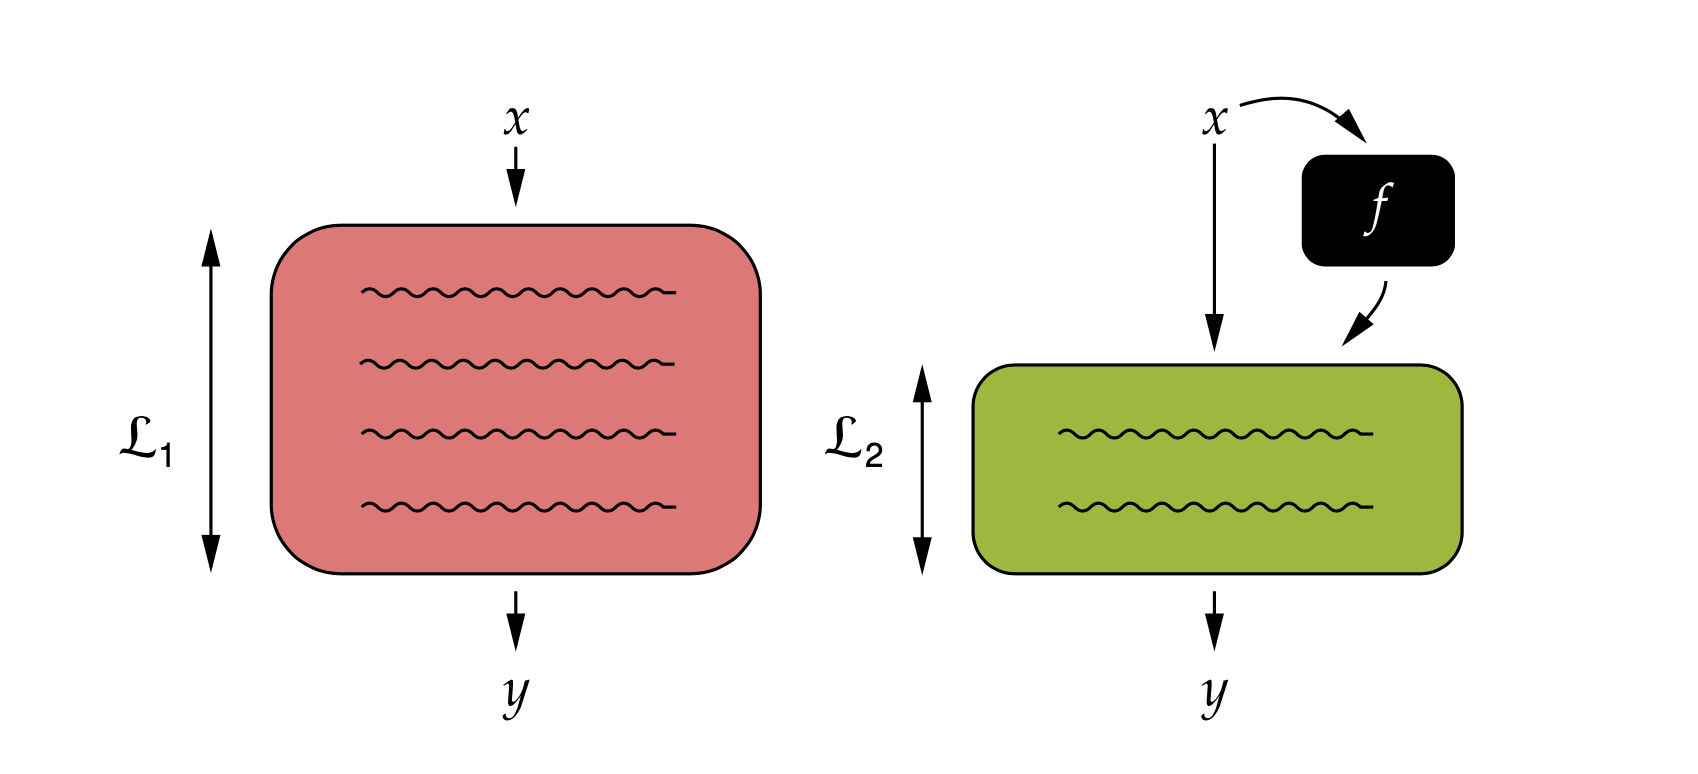
\includegraphics[width=\textwidth]{capability.png} 
                \caption{A capability $f$ is useful if it shortens the minimum program needed to perform a task, as measured by Minimum Description Lengths $\mathcal{L}_1$ and $\mathcal{L}_2$. To give a concrete example, if $x$ is a question and $y$ is an answer, then $f$ can be an oracle that answers relevant subquestions}
            \end{figure}
        \end{column}
    \end{columns}
\end{frame}

\begin{frame}
\frametitle{Formalisation}
\begin{itemize}
  \item Let $x_{1:N}$ be our data, $y_{1:N}$ -- corresponding labels.

  \item Let $\mathcal{L}(y_{1:N} | x_{1:N})$ be the length of the shortest program $P$ that maps $x \rightarrow y$, which is precisely data's \textbf{Kolmogorov complexity}.

  \item Let $f$ be the function that maps $x_n$ to a possibly helpful output $f (x_n)$, with $\mathcal{L}(y_{1:N} |x_{1:N},f)$ being the length of the shortest label-generating program when access to $f$ is given.
  \item We say $f(x)$ is \textbf{helpful} for building a good model of the data when
\end{itemize}
$$\mathcal{L}(y_{1:N} |x_{1:N},f) < \mathcal{L}(y_{1:N} | x_{1:N})$$

\begin{itemize}
  \item As P is often uncomputable, we can instead consider compressed version  $y_{1:N}$ along with \textbf{decompressing algorithm} that obtain $y_{1:N}$  given data and compressed  $y_{1:N}$. Then, to find $\mathcal{L}$, then, we find the length of the maximally compressed $y_{1:N}$, which is precisely MDL.
  \item In general, MDL is also uncomputable, but we can estimate it by \textbf{restricting the set of allowed compression algorithms}.
\end{itemize}

\end{frame}


\begin{frame}
	\frametitle{Online Coding}
	\begin{block}{Reminder}
            We had Alice and Bob who both have data $x_{1:N}$, but only Alice has labels $y_{1:N}$ and she wants to message them to Bob, spending as less bits as possible
	\end{block}
\begin{columns}[onlytextwidth]
        \begin{column}{0.3\textwidth}
            \begin{itemize}
                \item To examine how much $y_{1:N}$ can be compressed, we look at the minimum number of bits to send $y_{1:N}$.
                \item Alice and Bob both have model $p_{\theta_1}$.
            \end{itemize}
        \end{column}
        \begin{column}{0.7\textwidth}
            \begin{figure}
                \centering
                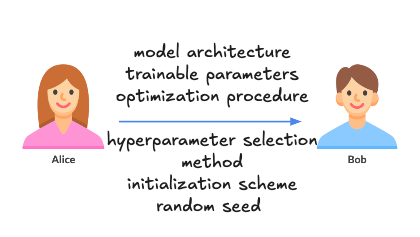
\includegraphics[width=\textwidth]{alice_bob.png} 
            \end{figure}
        \end{column}
    \end{columns}
    
\end{frame}

\begin{frame}{Algorithm}
    \begin{enumerate}
        \item Alice send each label $y_i$ one by one; Shannon has proved that $-\log p_{\theta_n}(y_n |x_n)$ bits are enough if Alice and Bob share $x_n$ and $p_{\theta_n}$.
        \item After Alice has sent Bob $y_n$, they both train a better model  $p_{\theta_{n +1}}(y|x)$ on the subset of data that Alice already messaged. The objective here is to shorten codes for future labels.

        The codelength for $y_{1:N}$ is:
        $$\mathcal{L}_p(y_{1:N} |x_{1:N}) = \sum_{n=1}^N -\log p_{\theta_n}(y_n |x_n)$$
        \item Overall, Alice' message consists of $\mathcal{L}_p(y_{1:N} |x_{1:N})$ bits + bits required to transmit information about the model.
    \end{enumerate}

    \begin{block}{Capability}
        If both Alice and Bob have $f$ to encode labels within the model $p_{\theta}(y|x,f)$, then f is considered helpful when the message is shorter with f than without it: 

        $$\mathcal{L}_p(y_{1:N} |x_{1:N},f) < \mathcal{L}_p(y_{1:N} | x_{1:N})$$
    \end{block}
\end{frame}

\begin{frame}{Practical tricks}
   As $\mathcal{L}_p(y_{1:N} |x_{1:N})$ is quadratic in $N$, it is suggested to use \textbf{block-wise coding}, meaning data is sent in discrete blocks rather than as a continuous stream. Therefore, Alice and Bob only train the model upon having sent $0 = t_0 <t_1 < \dots < t_S = N$ labels. 

   More specifically, Alice sends all labels in a ``block'' $y_{t_s+1:t_{s+1}}$ at once using $p_{\theta_{t_s}}$. As $p_{\theta_0}$ has no training data, it has a uniform prior.
    \begin{block}{Codelength with blocks}
         $$\overline{\mathcal{L}}_p(y_{1:N} |x_{1:N}) = \sum_{s=0}^S \sum_{n=t_s +1}^{t_{s +1}} -\log p_{\theta_{t_s}}(y_n |x_n)$$

    \end{block}
  



    Also, to alleviate the \textbf{sensitivity} to particular learning algorithm, authors suggest to ensamble many model classes. Alice train $M$ models of different classes and send the next block’s labels using the model that gives the shortest codelength. To tell Bob which model to use to decompress a block’s labels, Alice also sends $\log M$ bits per block, overall adding $(S  - 1) \log M$ to MDL.
\end{frame}

\begin{frame}
	\frametitle{Results}
\begin{columns}[onlytextwidth]
        \begin{column}{0.5\textwidth}
            \begin{figure}
                \centering
                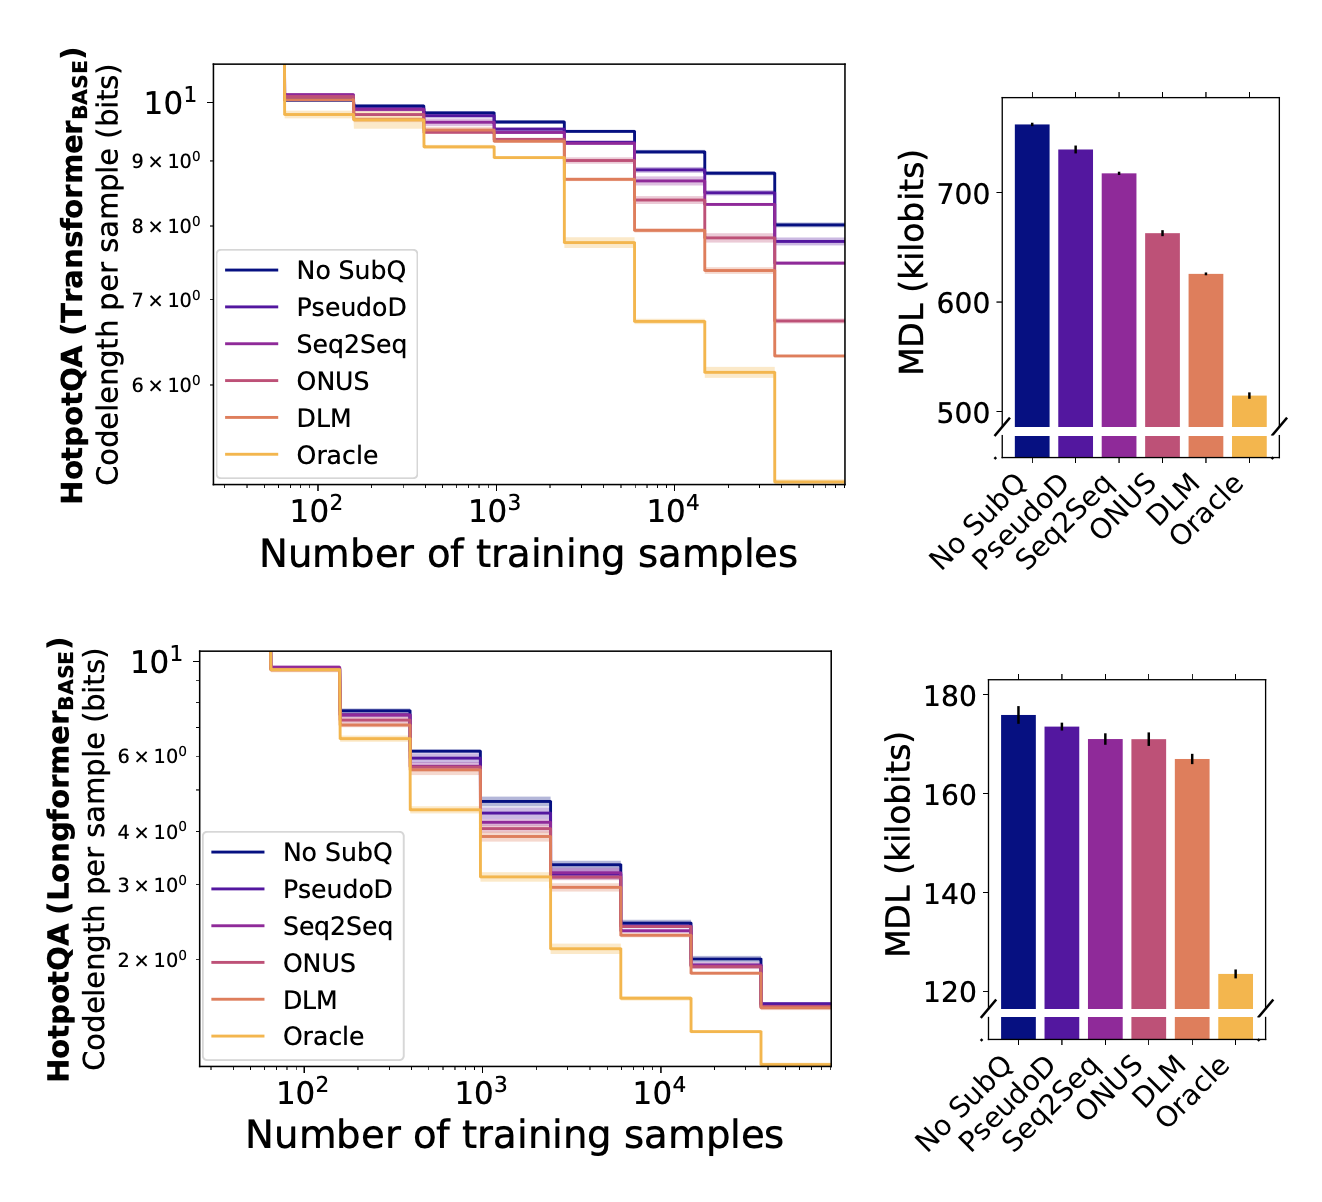
\includegraphics[width=\textwidth]{hotpotqa.png} 
                \caption{HotPotQA have a question, two supporting Wikipedia paragraphs and 8 distractors}
            \end{figure} 
        \end{column}
        \begin{column}{0.5\textwidth}
            \begin{figure}
                \centering
                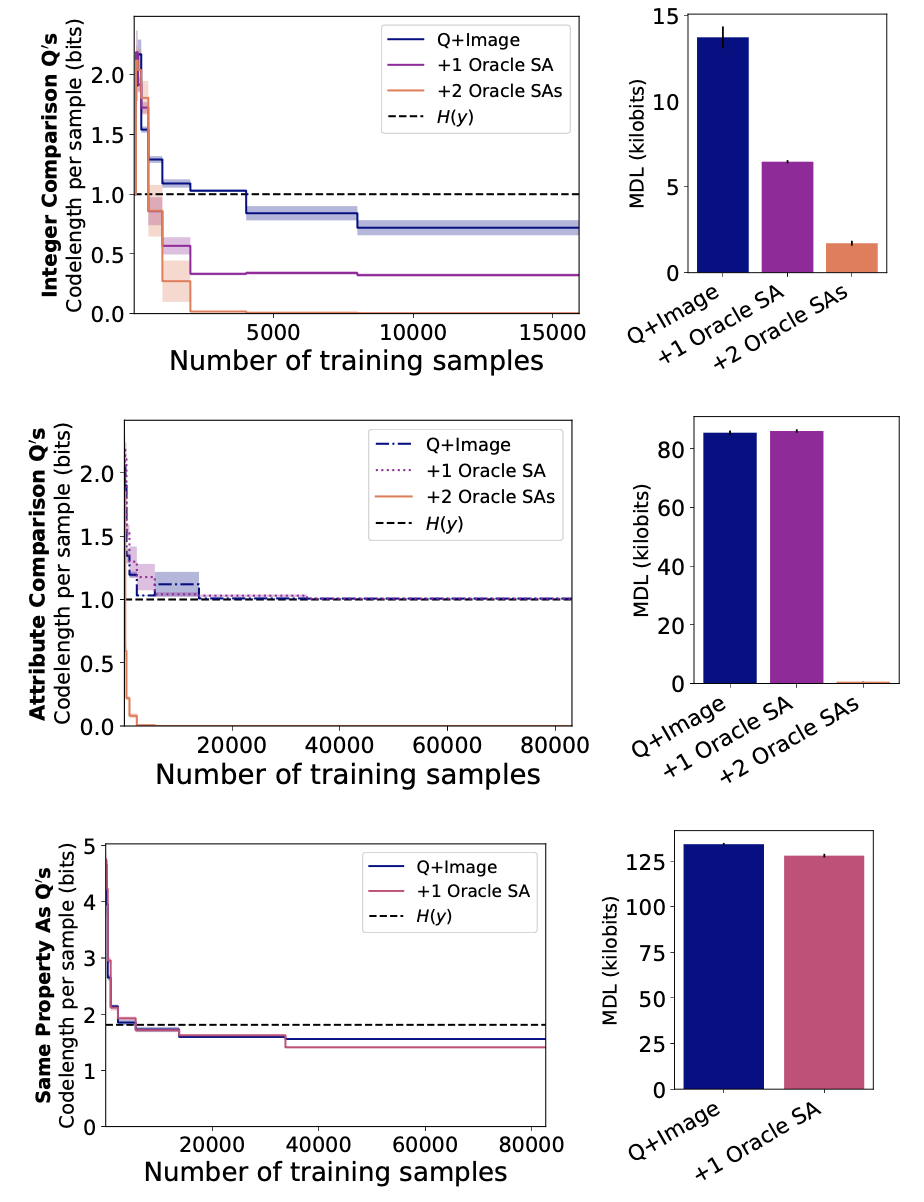
\includegraphics[width=0.9\textwidth]{clevr.png} 
                \caption{CLEVR: image-based QA system}
            \end{figure}
        \end{column}
    \end{columns}
    
\end{frame}


\begin{frame}{Conclusions}
    \begin{itemize}
        \item Rissanen Data Analysis is empirically useful for examining the characteristics of datasets, revealing biases and capabilities that can be beneficial for different tasks;
        \item MDL decreases when models were given answers to subquestions in image-based question-answering tasks;
        \item On HotPotQA, RDA shows that decomposing questions into subquestions is indeed helpful;
        \item Answering subquestions significantly aids in resolving complex queries, such as comparing quantities and attributes of objects.
        \item Also in work authors analyse how adding various explanations, word order and presence of various POS (Part-Of-Speech) affect MDL. They discover that word order is important, adjectives are crucial for sentiment analysis, while verbs play a key role in linguistic acceptability tasks and explanations are indeed helpful to reduce MDL.
    \end{itemize}
\end{frame}

\end{document}